\graphicspath{ {Figures/Pileup/Multiplier/} {Figures/Pileup/Phase/} {Figures/RandomSeeds/FitStartScans/} {Figures/RandomSeeds/FitIterations/} {Figures/Miscellaneous/} {Figures/CBO/Shape/} {Figures/CBO/LifetimeScan/} {Figures/Gain/InFill/} }

\chapter{Systematic Uncertainty Evaluations}

\section{Sensitivity of \texorpdfstring{$\omega_{a}$}{} to gain corrections}

	\subsection{In-Fill Gain}

		As positrons hit the calorimeters throughout the fill, there will be a gain sag response such that the energy of detected positrons changes throughout the fill, dropping at first and then rising exponentially back up to their true values. This changing energy response will lead to a systematic error on R, as positrons with mis-measured energies near the energy threshold are excluded from the fit. This gain sag is corrected for in the Recon West code, before I fill my histograms. Due to the way I've constructed my analysis code, it's not so simple to modify the reconstruction code and create new histograms quickly. Such a process would require the rebuilding of many sets of new cluster root trees, and then making histograms from those. As a faster way of getting at the in fill gain systematic error, I've instead chosen to apply a gain sag function to the incoming energy-corrected clusters. This allows me to scan over gain sag function parameters and only run off one set of trees, as I've been doing for all systematic studies.

		(Should this bit be in the analysis procedures chapter?) The in-fill gain sag function was determined by Matthias Smith and the laser team as shown in DocDB 14077. (Cite or link?) The function goes as  
			\begin{gather}
				E = E_{0}(1 - A \cdot e^{-(t-t_{offset})/\tau}),
			\label{Eqn:GainSag}
			\end{gather}
		where $E_{0}$ is the orginal energy of the positron cluster, A is the amplitude factor on the gain sag function, $\tau$ the lifetime, and then $t_{offset}$ the shift of the function from 0. It is this function that is inverted and applied to the clusters in the reconstruction. I apply a function of the same form in my own code before filling hits into histograms, in essence undoing the reconstruction gain correction as a way to measure the in-fill gain sag effect on R.

		\begin{figure}[h]
			\centering
			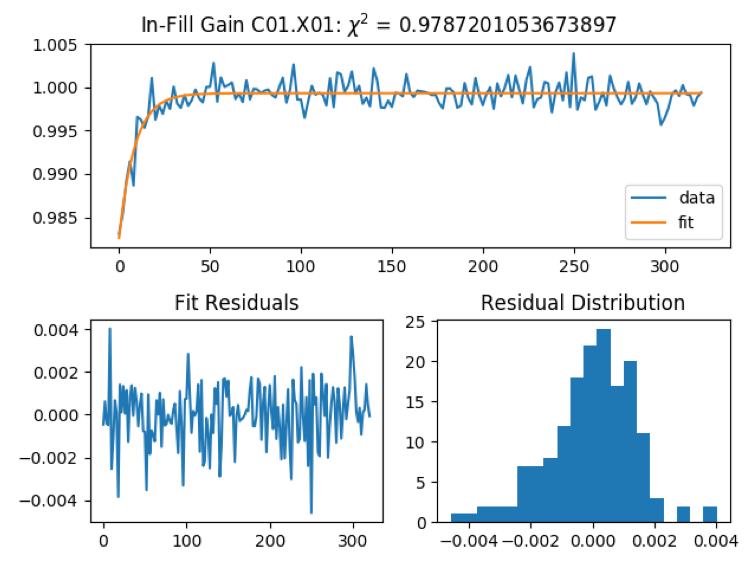
\includegraphics[width=.8\textwidth]{MatthiasInFill}
		    \caption[MatthiasInFill]{The top plot shows the in-fill gain sag function in orange from a fit to data in blue, for crystal 1 in calorimeter 1. The gain sag can be modeled effectively by a simple exponential function. By $\SI{30}{\mu s}$ the change in energy response is nearly only .1\%. (Might want to look up these exact numbers.) The bottom two plots show the residuals of the fit. Plot made by Matthias Smith.}
		    \label{Fig:MatthiasInFill}
		\end{figure}

		There are some simplifications and assumptions I've made when applying said gain sag function in my own code. First is that while in the reconstruction code each crystal of each calorimeter has its own singular in-fill gain function, one of which is shown in Figure \ref{Fig:MatthiasInFill}, I apply a global gain sag function to all incoming clusters. Secondly the default parameters for the gain sag function are simply eyeballed from the fcl file where all crystal parameters are stored. These values are 0.03 for the amplitude, $\SI{6.7}{\mu s}$ for the lifetime, and $\SI{3.907}{\mu s}$ for the offset. (Once the latest dataset is available I will need to come up with a better way to apply this gain sag function, either with multiple functions per crystal or with parameters that are actual averages. For now it's fine though to get words on the paper.) Finally, I apply this gain sag function after I apply the artificial deadtime to the incoming clusters, due to code restrictions. This should be a small effect. These assumptions I believe should be okay as long as I take my systematic errors conservatively.

		\begin{figure}[]
		\centering
		    \begin{subfigure}[t]{0.45\textwidth}
			    \centering
				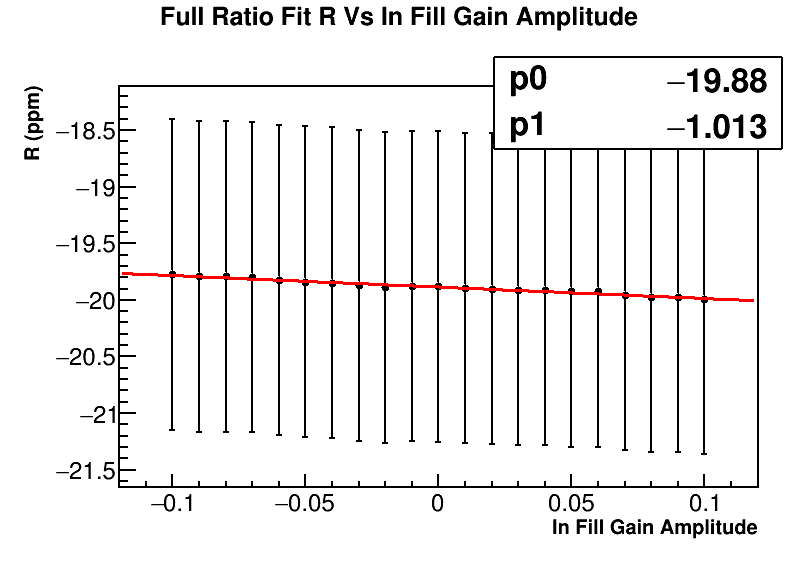
\includegraphics[width=\textwidth]{RatioCBO_R_Vs_InFillGainAmplitude_Canv}
			    \caption{Plotted is R vs the amplitude parameter in the gain sag function. The slope is -1.013 ppm per unit amplitude.}
		    \end{subfigure}
		    \hspace{4mm}
		    \begin{subfigure}[t]{0.45\textwidth}
			    \centering
				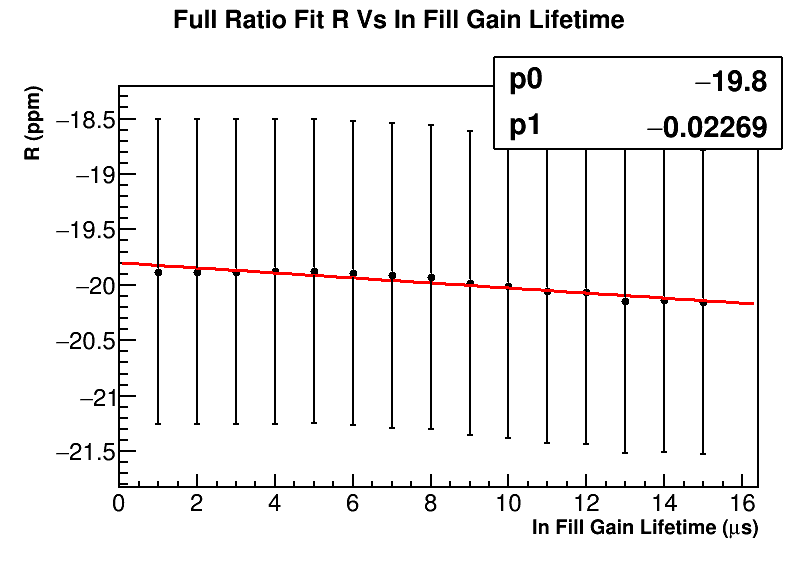
\includegraphics[width=\textwidth]{RatioCBO_R_Vs_InFillGainLifetime_Canv}
			    \caption{Plotted is R vs the lifetime parameter in the gain sag function. The slope is -0.02269 ppm per $\mu s$.}
		    \end{subfigure}% %you need this % here to add spacing between subfigures
		    \vspace{4mm}
		    \begin{subfigure}[t]{0.45\textwidth}
			    \centering
				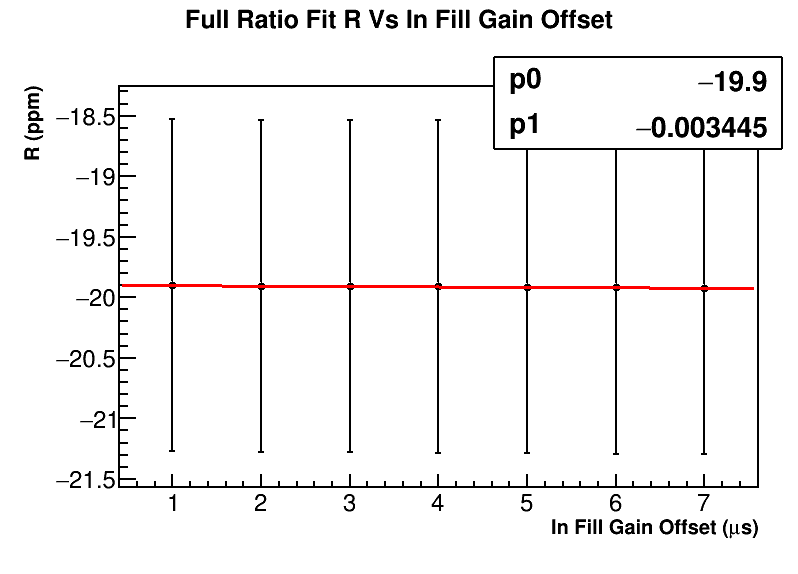
\includegraphics[width=\textwidth]{RatioCBO_R_Vs_InFillGainOffset_Canv}
			    \caption{Plotted is R vs the offset parameter in the gain sag function. The slope is -0.0034 ppm per $\mu s$.}
		    \end{subfigure}% %you need this % here to add spacing between subfigures
		\caption[InFillGain]{Plotted is fitted R values vs gain sag function parameters. In each case I scanned over ranges approximately centered around the eyeballed average values.}
		\label{Fig:InFillGain}
		\end{figure}

		To calculate the systematic error, I simply scan over the gain sag function parameters and observe the changes in R. This includes scans over the amplitude, lifetime, and offset as described in \ref{Eqn:GainSag}, and shown in Figure \ref{Fig:InFillGain}. I calculate the systematic error on R as the quadrature sum of the separate pieces as 
		\begin{align}
			\delta R_{A} &= \delta\alpha_{A} \times \frac{dR}{d\alpha_{A}}, \\
			\delta R_{\tau} &= \delta\alpha_{\tau} \times \frac{dR}{d\alpha_{\tau}}, \\
			\delta R_{offset} &= \delta\alpha_{offset} \times \frac{dR}{d\alpha_{offset}},
		\end{align}
		where $\delta\alpha_{A}$, $\delta\alpha_{\tau}$, and $\delta\alpha_{offset}$ are the uncertainties on the gain sag amplitude, lifetime, and offset respectively. I take the uncertainty on the amplitude very conservatively at 1\%, leading to a systematic error on R of $0.01 \times \SI{1.013}{ppm} = \SI{10.1}{ppb}$. I take the uncertainty on the lifetime very conservatively at $\SI{1}{\mu s}$, leading to a systematic error on R of $1 \times \SI{22.7}{ppb} = \SI{22.7}{ppb}$. Finally the slope for the offset parameter is very flat, and that combined with a very uniform array of values for the offset parameter in the reconstruction (indicative of a very small uncertainty), means that the systematic error on R is negligible. Therefore I ignore the offset parameter and add the amplitude and lifetime errors in quadrature to produce a systematic error on R of 24.8 ppb. (The uncertainty on the parameters would be the fit errors on the parameter I think, except for the fact that I'm using a global gain sag function as opposed to crystal functions, meaning the uncertainty might be the spread in parameters. I'm not entirely sure. Maybe ask Matthias/Laser team and James.)

	\subsection{Short Term Double Pulse (SDTP)}


\section{Sensitivity of \texorpdfstring{$\omega_{a}$}{} to pileup}

	The systematic error on R due to the pileup construction consists primarily of two parts, the error due to misconstruction of the amplitude and the phase of the pileup. The error due to the amplitude misconstruction was calculated by scanning over a pileup multiplier parameter, from 90\% of the calculated pileup amplitude to 110\%, as shown in Figure \ref{fig:PileupMultiplier}. The sensitivity of R to the amplitude was determined to be 509.1 ppb per unit amplitude. The uncertainty of the pileup amplitude construction was determined by fitting a parabola to the \chisq as a function of the pileup amplitude, and taking the width of that parabola as the uncertainty. This width is determined as the distance in X for the \chisq to rise by 1 from the minimum, also calculated as $\sqrt{2/(\chi^{2})''}$.

	\begin{figure}[h]
	\centering
	    \begin{subfigure}[t]{0.45\textwidth}
		    \centering
			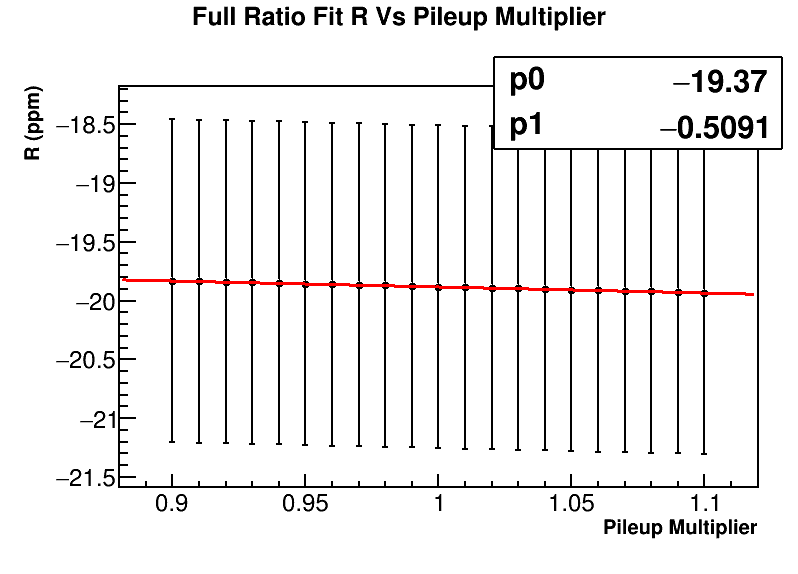
\includegraphics[width=\textwidth]{RatioCBO_R_Vs_PileupMultiplier_Canv}
		    \caption{Sensitivity of R vs the pileup amplitude. The slope is -509.1 ppb per unit amplitude.}
	    \end{subfigure}
	    \hspace{4mm}
	    \begin{subfigure}[t]{0.45\textwidth}
		    \centering
			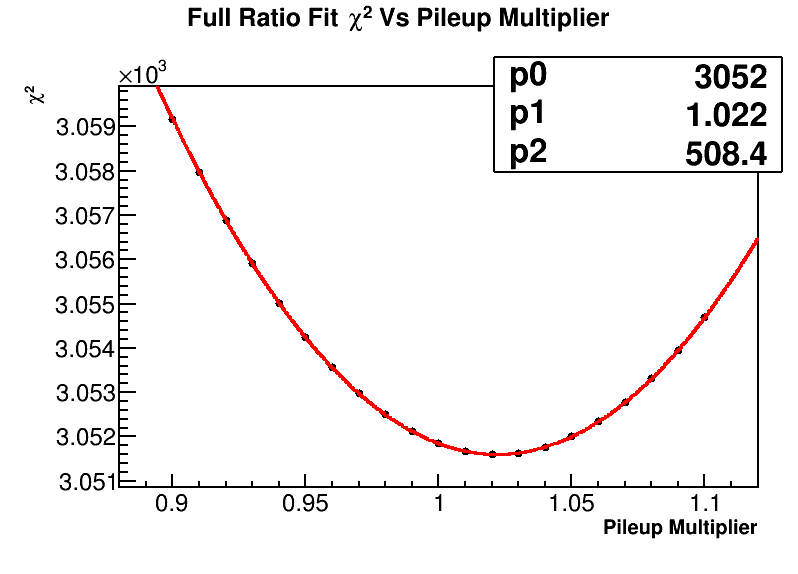
\includegraphics[width=\textwidth]{RatioCBO_Chi2_Vs_PileupMultiplier_Canv}
		    \caption{Plotted is the fitted \chisq vs the pileup amplitude. The fit equation used was $p2 \times (x - p1)^{2} + p0.$ The minimum therefore lies at 1.022.}
	    \end{subfigure}
	\caption[PileupMultiplier]{The significant plots to determine the pileup amplitude systematic error.}
	\label{fig:PileupMultiplier}
	\end{figure}

	This corresponds to an uncertainty of $\sqrt{1/508.4} = 0.0444$ or 4.44\%. The minimum of the \chisq plot of 1.022 lies at approximately .5$\sigma$ away from 1, which is consistent and nice to see. Then, calculating the systematic error on R due to the pileup amplitude construction as 
		\begin{align}
			\delta R_{pm} = \delta\alpha_{pm} \times \frac{dR}{d\alpha_{pm}}
		\end{align}
	where $\delta\alpha_{pm}$ is the uncertainty on the pileup amplitude, the systematic error on R is calculated as $0.0444 \times \SI{509.1}{ppb} = \SI{22.6}{ppb}$.

	Another technique to estimate the uncertainty of the pileup amplitude construction is to look at the offset of the high energy tail of the pileup subtracted energy spectrum from zero. Because however I've applied only the doublet correction, I know that the shape of the pileup spectrum is wrong by some amount, as evidenced in \ref{fig:AddedEnergies}. While the pileup itself can multiplied by some scaling factor other than 1 in order to align the energy spectra slightly better, because the shape of the pileup correction is imperfect the offset calculation I believe is the wrong way to go about calculating this uncertainty in my case. The shape can be fixed by including the triplets and the doublet contamination in the shadow method, but that work is incomplete. Since the triplets are a 1\% effect relative to the doublets, and the contamination is of the same order, I believe the uncertainty of 4.44\% conservatively includes for this mismatch in shape and the omission of the triplets. Regardless, since the statistics of the 60H dataset is much larger than the order of the systematic effect for the pileup construction ($\mathcal{O}$(1 ppm) vs $\mathcal{O}$(10 ppb)), this is a fine assumption.

	\begin{figure}[h]
		\centering
		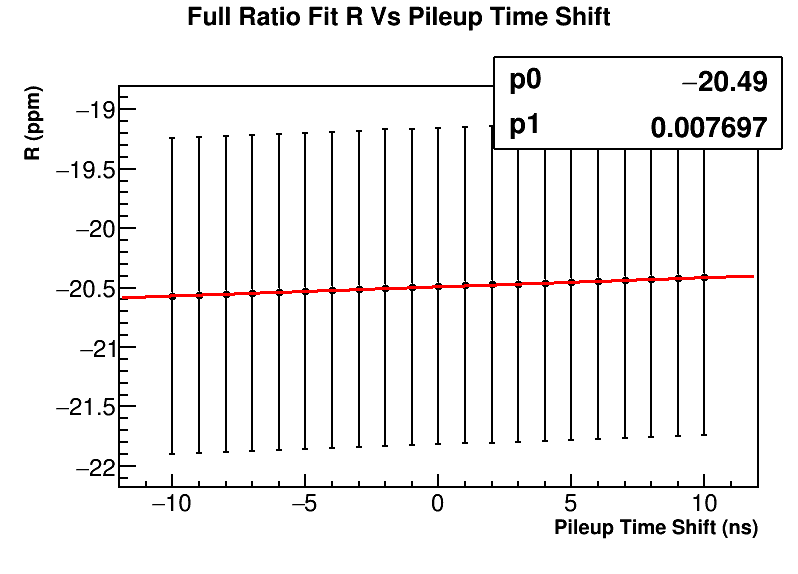
\includegraphics[width=.5\textwidth]{RatioCBO_R_Vs_PileupTimeShift_Canv}
	    \caption[PileupPhase]{Sensitivity of R vs the pileup phase. The slope is 8.571 ppb per ns.}
	    \label{fig:PileupPhase}
	\end{figure}

	The error on R due to the pileup phase construction was calculated by scanning over a pileup time shift parameter, where the pileup spectrum was shifted in time by some amount before subtraction. The sensitivity of R to this parameter is shown in Figure \ref{fig:PileupPhase}. It is extremely unlikely that the entire pileup spectrum could be shifted by the offsets shown here, so this is a conservative estimate of the effect of the pileup phase on R. Another factor that the phase depends on is the energy dependence of the constructed pileup pulses, calculated as just the sum of the singlets. If the energy is miscalculated then the phase of the included pulses will be off. However, because the spatial separation is turned off in the reconstruction clustering, this is a small effect for my pileup construction method. Similarly, in the near future the Short Term Double Pulse (STDP) improvement to the laser calibration will be included also reducing this effect. For these reasons and due to the conservative nature of my phase error estimation, I leave such effects out. I then calculate the phase error as 
		\begin{align}
			\delta R_{pp} = \delta\alpha_{pp} \times \frac{dR}{d\alpha_{pp}}
		\end{align}
	where $\delta\alpha_{pp}$ is the uncertainty on the pileup phase. I once again very conservatively estimate the uncertainty on the pileup phase as half the artificial deadtime at 3 ns. The systematic error on R is then calculated as $\SI{3}{ns} \times \SI{8.571}{ppb/ns} = \SI{25.7}{ppb}$. This is a very conservative estimate which is fine once again because of the comparison of order of statistics vs the systematic effect.

	\begin{figure}[]
		\centering
		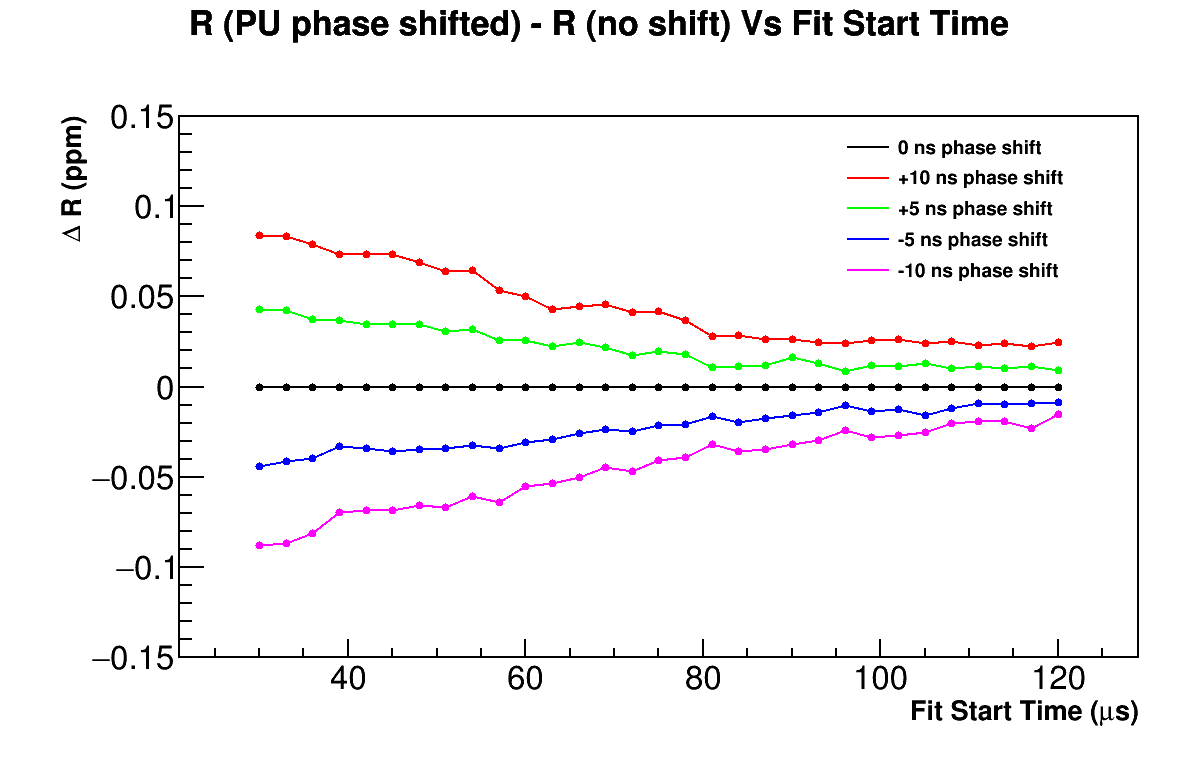
\includegraphics[width=.8\textwidth]{pileupTimeShiftComparison}
	    \caption[PileupTimeShiftFS]{Plotted is $\Delta R$ between pileup time shifted and unshifted results vs fit start time. The black line and points are by definition 0. As the fit start time increases and the pileup reduces, the $\Delta R$ points converge to zero as they should.}
	    \label{fig:PileupTimeShiftFS}
	\end{figure}

	Adding these two errors in quadrature results in a systematic error on R due to the pileup as 34.2 ppb.



\section{Sensitivity of \texorpdfstring{$\omega_{a}$}{} to lost muon function shape}

\section{Sensitivity of \texorpdfstring{$\omega_{a}$}{} to CBO function}

	\subsection{CBO Shape}

		If the shape of the CBO in the fit function is wrong, then there will be a systematic error on R. Because I get good fits and the CBO parameters are stable vs fit start time, the possbile changes to the envelope are limited, compared to the envelope used as shown in Equation \ref{eqn:CBO}. Possible changes to the envelope include those functions as shown in Figure \ref{fig:CBOShapeAmplitude}, an exponential plus a constant and then an exponential times another oscillatory term. Both new envelopes were determined from tracker analysis fits to the CBO amplitude. Both changes to the envelope amplitude were tried in the fitting function, with changes in R of $\SI{-21.1}{ppb}$ and $\SI{-9.6}{ppb}$ respectively, though neither showed any improvement in the fit. (In the latter the period of the oscillatory term was fixed and the other parameters were allowed to float.) I take the latter value of $\SI{21.1}{ppb}$ as the systematic error on R due to the shape.

		\begin{figure}[]
			\centering
			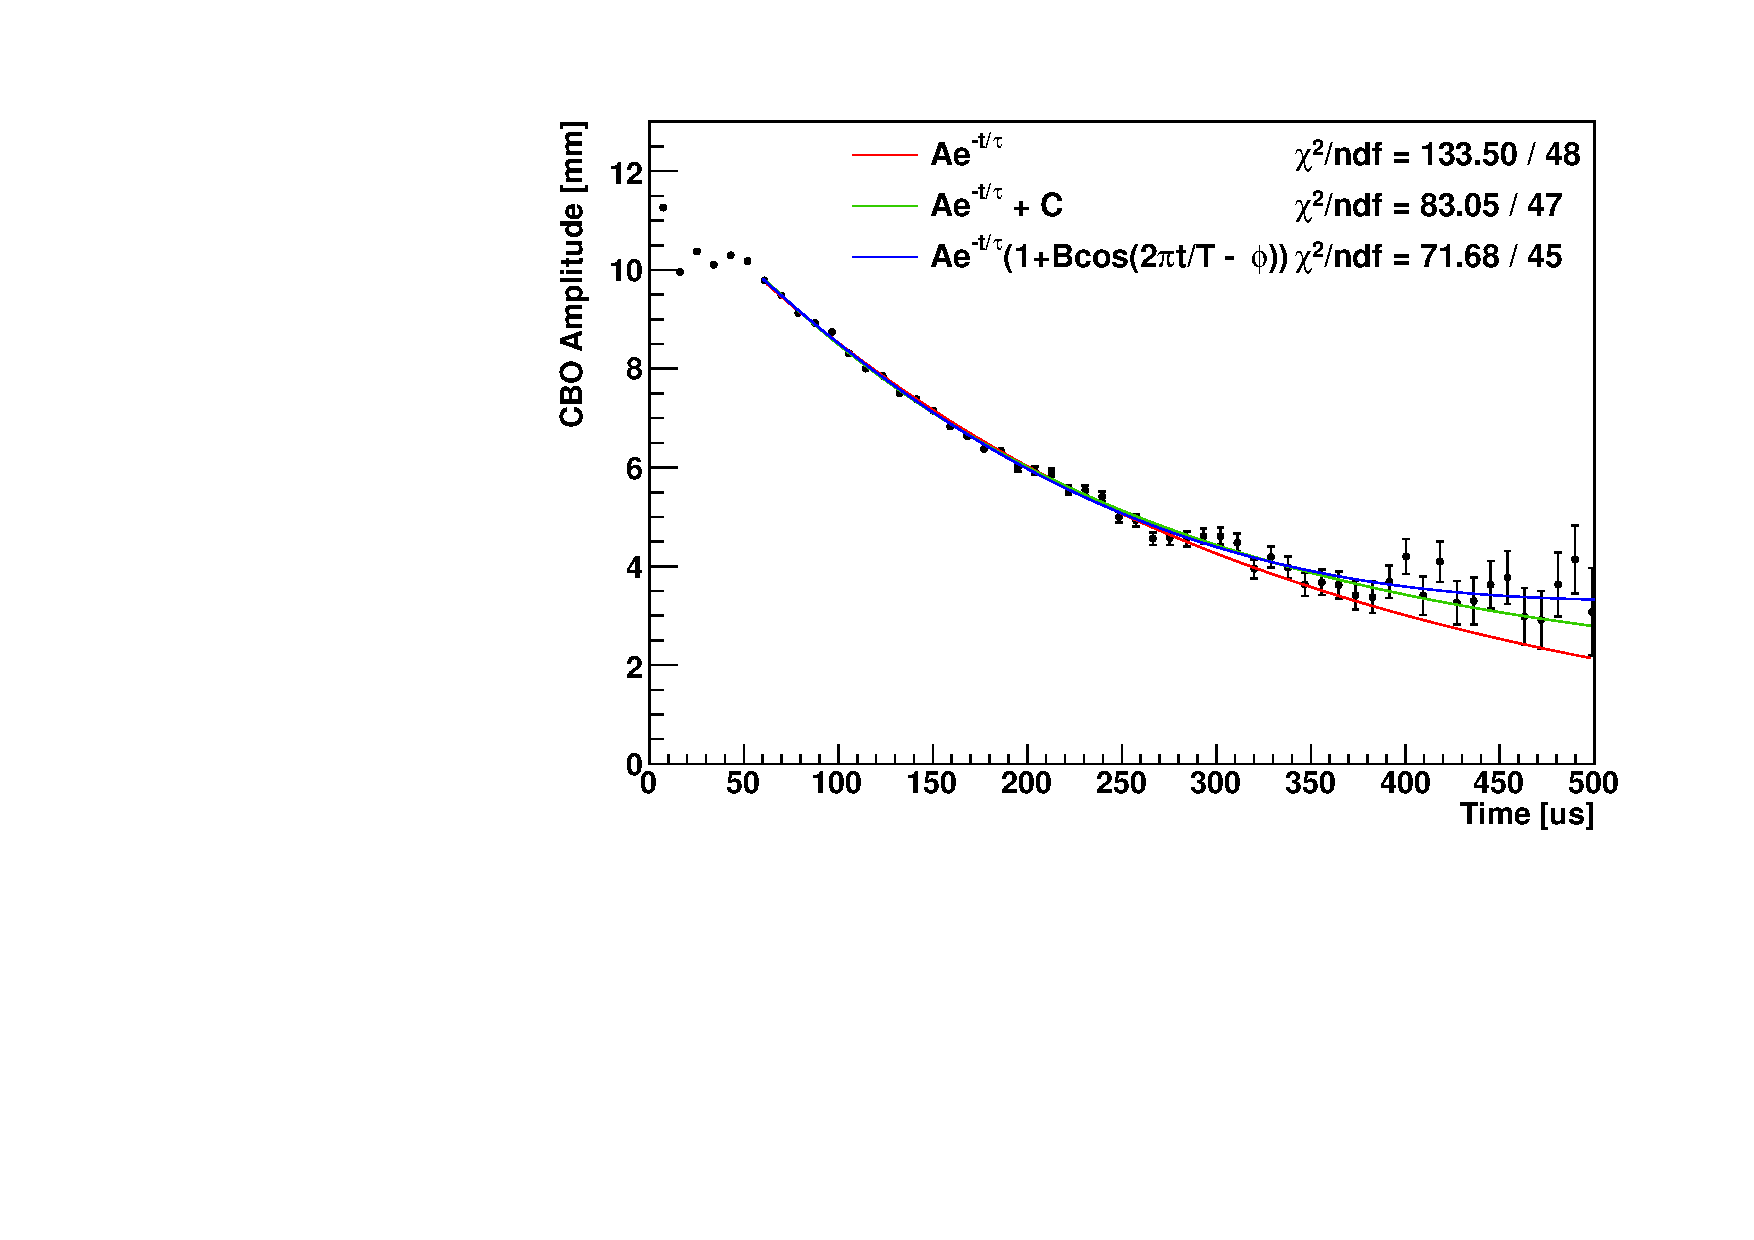
\includegraphics[width=.7\textwidth]{AmplFitOptions}
		    \caption[CBOShapeAmplitude]{Plotted is the CBO amplitude as a function of time from the tracker analysis. Three separate fit functions were used with varying degrees of success to characterize the envelope shape of the CBO (excepting the cosine modulation part). A Gaussian fit was tried with no success. The amplitude isn't fully understood at early times. The period T/$2\pi$ has a value of $\SI{114.5}{\mu s}$. Plot producd by James Mott.}
		    \label{fig:CBOShapeAmplitude}
		\end{figure}

	\subsection{CBO Frequency}

		What about systematic errors for the cbo frequency? Should this be provided from the trackers or something that I do?

	\subsection{CBO Lifetime}

		Because the CBO lifetime has been fixed in the fit, there is a systematic error on R. Scanning over various values of the fixed CBO lifetime allows this error to be calculated. The resulting curve of R vs the CBO lifetime turns out not to be linear, as shown in Figure \ref{fig:CBOLifetime}. Taking the uncertainty on the CBO lifetime as the error produced by the T Method fit, approximately $\SI{16}{\mu s}$, and looking at the change in R for CBO lifetime values of $180 \pm \SI{16}{\mu s}$, the systematic error on R is taken as the larger of the two at 12.1 ppb.

		\begin{figure}[]
			\centering
			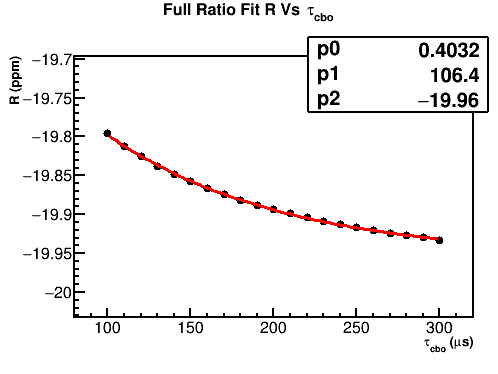
\includegraphics[width=.6\textwidth]{RatioCBO_R_Vs_tau_cbo_Canv}
		    \caption[CBOLifetime]{Plotted is the fitted R value as a function of the CBO lifetime, which has been fixed in the full ratio fit. The error bars have been removed from the plot in order to show the shape of the curve better. The points have been fitted to an exponential function which lines up nicely, $p_{0} e^{-t/p_{1}} + p_{2}$.}
		    \label{fig:CBOLifetime}
		\end{figure}





\section{Sensitivity of \texorpdfstring{$\omega_{a}$}{} to VW function}

\section{Sensitivity of \texorpdfstring{$\omega_{a}$}{} to various effects}

	\subsection{\gmtwo Period Guess}

		To perform the ratio method, the \gmtwo period needs to be known a priori to high precision. By scanning over various \gmtwo period guesses the dependence of R on $T_{a}$ can be determined, as shown in Figure \ref{fig:gm2PeriodGuess}. The systematic error can then be calculated as 
			\begin{align}
				\delta R_{period} = \delta\alpha_{period} \times \frac{dR}{d\alpha_{period}}
			\end{align}
		where $\delta\alpha_{period}$ is the uncertainty on $T_{a}$. Very conservatively taking the uncertainty as 10 ppm, the systematic error on R is calcualted as $\SI{10}{ppm} \times \SI{1.62e-4}{ppm/ppm} = \SI{1.62}{ppb}$, which is completely negligible.

		\begin{figure}[]
			\centering
			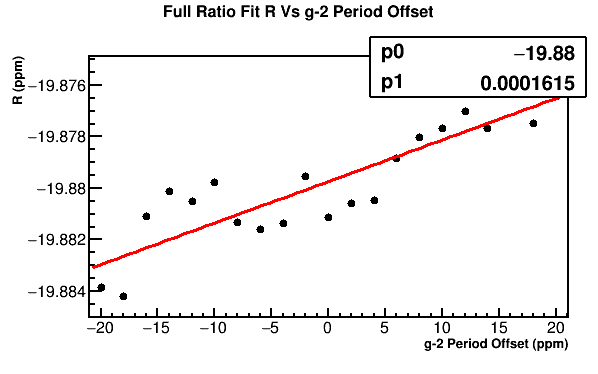
\includegraphics[width=.6\textwidth]{RatioCBO_R_Vs_gm2PeriodGuess_Canv}
		    \caption[gm2PeriodGuess]{Fitted R value as a function of the ppm level offset from the guess used for the \gmtwo period, \ref{eq:Ta}. Error bars have been removed from this plot, otherwise it appears as a flat line. The slope is .16 ppb per ppm offset in $T_{a}$.}
		    \label{fig:gm2PeriodGuess}
		\end{figure}


	\subsection{Bin Width}

		The systematic uncertainty from the bin width, chosen to eliminate the fast rotation signal, was calculated by performing the histogramming and fitting stages with varying values of bin widths. The systematic uncertainty is taken as the RMS spread of the fitted R values. As shown in Figure \ref{fig:BinWidth} it is 44.5 ppb.

		\begin{figure}[]
			\centering
			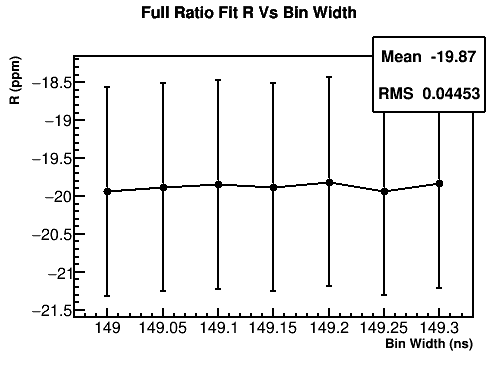
\includegraphics[width=.6\textwidth]{BinWidthComparison}
		    \caption[BinWidth]{Plotted are fitted R values for varying bin widths ranging from 149.00 ns to 149.30 ns in steps of 5 ns.}
		    \label{fig:BinWidth}
		\end{figure}

	\subsection{Randomization}

		I'm not sure what the systematic error due to the randomization should be. I'm also not sure what I should take as my final answer for R. Would it just be the average of all the random seeds?

		\begin{figure}[]
		\centering
		    \begin{subfigure}[t]{0.45\textwidth}
			    \centering
				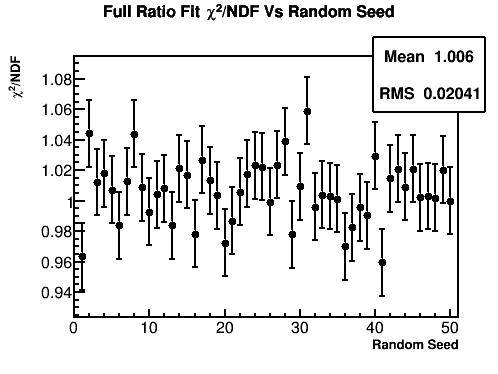
\includegraphics[width=\textwidth]{RatioCBO_Chi2NDF_Vs_Iter_Canv}
			    \caption{\chisq/NDF vs random seed number.}
		    \end{subfigure}
		    \begin{subfigure}[t]{0.45\textwidth}
			    \centering
				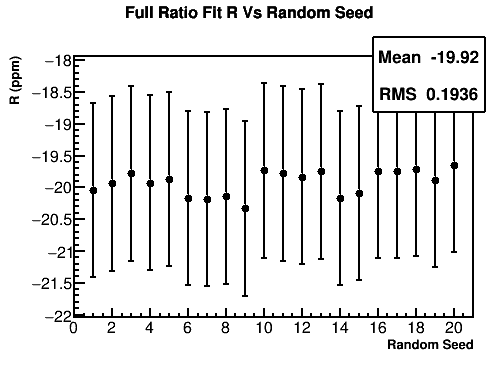
\includegraphics[width=\textwidth]{RatioCBO_R_Vs_Iter_Canv}
			    \caption{R vs random seed number.}
		    \end{subfigure}% %you need this % here to add spacing between subfigures
		\caption[RandomSeeds]{Plotted is the \chisq/NDF and fitted R value for 20 random seeds.}
		\label{fig:RandomSeeds}
		\end{figure}

		\begin{figure}[]
		\centering
		    \begin{subfigure}[t]{0.45\textwidth}
			    \centering
				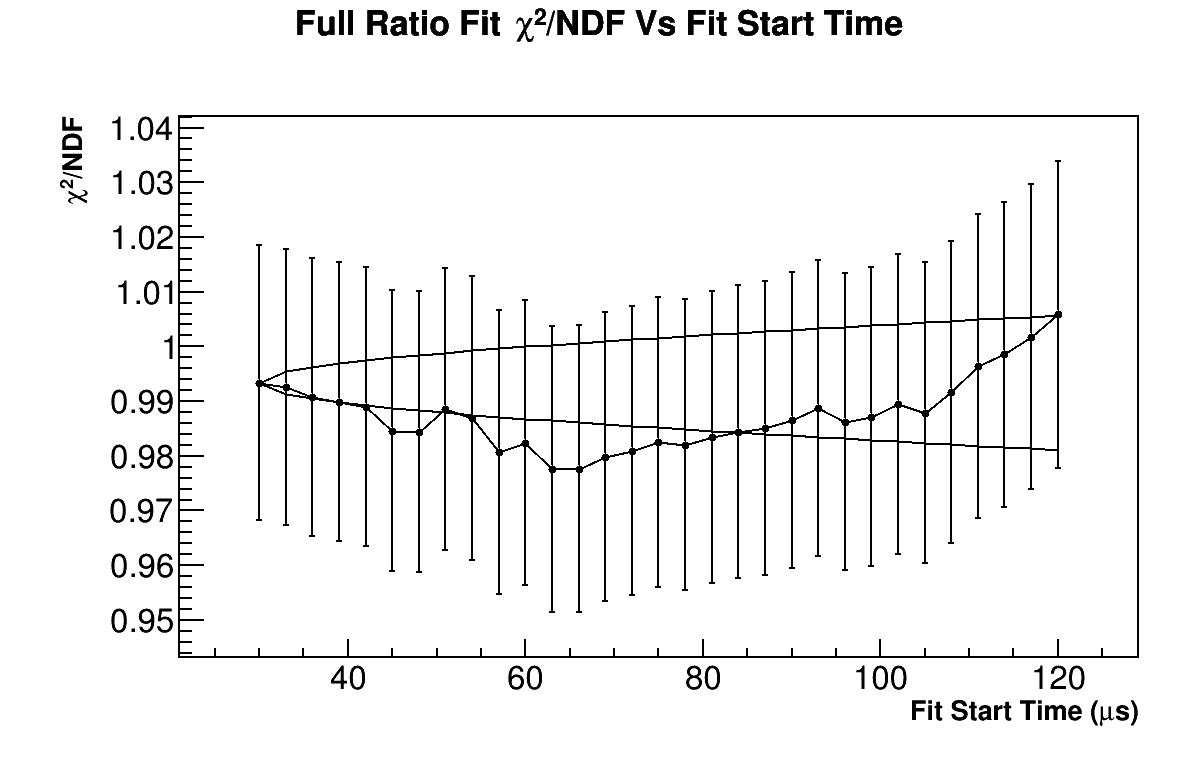
\includegraphics[width=\textwidth]{RatioCBO_Chi2NDF_Vs_FS_canv-Seed0}
			    \caption{Seed 1}
		    \end{subfigure}
		    \begin{subfigure}[t]{0.45\textwidth}
			    \centering
				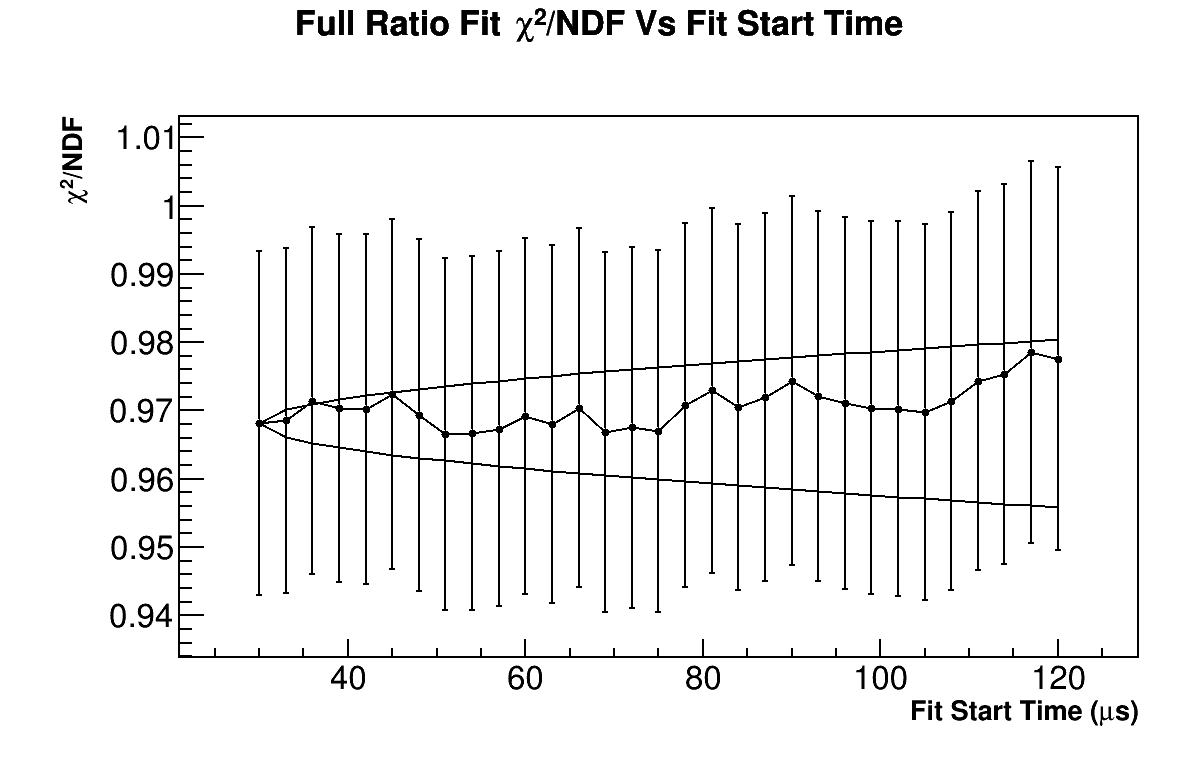
\includegraphics[width=\textwidth]{RatioCBO_Chi2NDF_Vs_FS_canv-Seed5}
			    \caption{Seed 2}
		    \end{subfigure}% %you need this % here to add spacing between subfigures
		    \vspace{4mm}
		    \begin{subfigure}[t]{0.45\textwidth}
			    \centering
				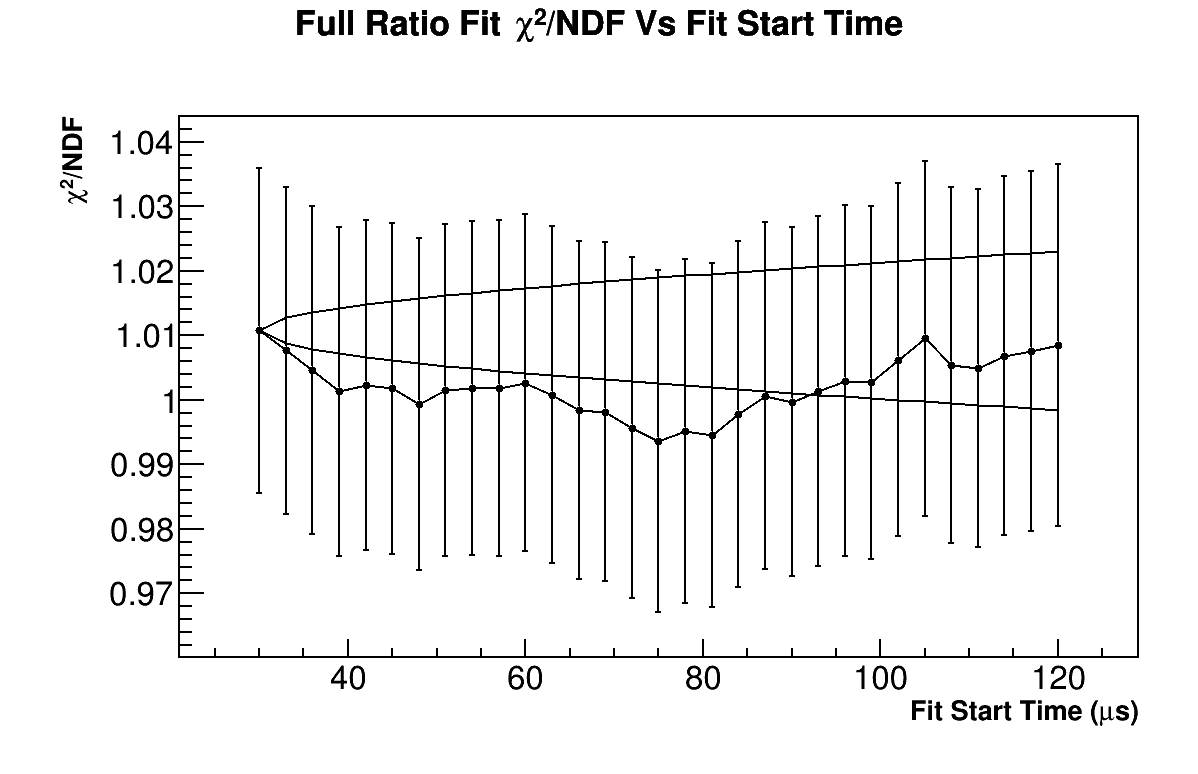
\includegraphics[width=\textwidth]{RatioCBO_Chi2NDF_Vs_FS_canv-Seed12}
			    \caption{Seed 3}
		    \end{subfigure}
		    \begin{subfigure}[t]{0.45\textwidth}
			    \centering
				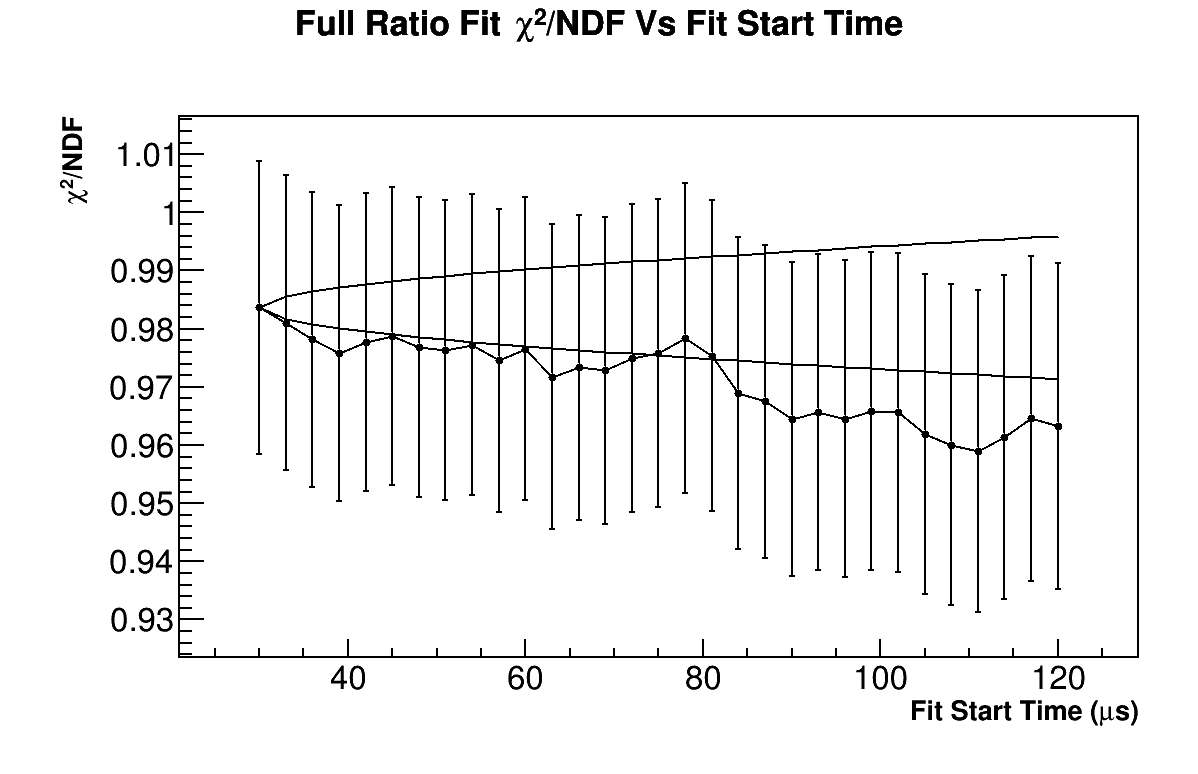
\includegraphics[width=\textwidth]{RatioCBO_Chi2NDF_Vs_FS_canv-Seed18}
			    \caption{Seed 4}
		    \end{subfigure}% %you need this % here to add spacing between subfigures
		\caption[RandomSeedFitStartScans]{Fit start time scans for the \chisq for four random seeds of the randomization of the same dataset. Compare to Figure \ref{fig:RatioCBO_Chi2NDF_Vs_FS_canv}. Note how the scans rise and fall at different points but are all consistent with the statistical bands.}
		\label{fig:RandomSeedFitStartScans}
		\end{figure}



\section{Final Systematic Uncertainty Table}


\begin{table}[H]
\setlength\tabcolsep{0pt}
\begin{tabular*}{\linewidth}{@{\extracolsep{\fill}}lS{c}}
  \toprule
    Systematic Error & 60H      \\
  \midrule
	Gain(+)    	     &  24.8  \\
	Pileup     	     &  34.2  \\
	Lost Muons       &        \\
	CBO(+)   		 &  24.3  \\
	VW 			     &        \\
	Bin Width        &  44.5  \\
	Randomization    &        \\
	Other   	     &        \\
  \bottomrule
\end{tabular*}
\caption{}
\end{table}



\section{Final Results}
